 %\vspace{-10pt}
 \section{Experiments} \label{sec:experiments}
 \vspace{-4pt}

 \begin{figure}[!t]
 \vspace{-2.3cm}
\centering
\begin{minipage}[c]{.45\linewidth}
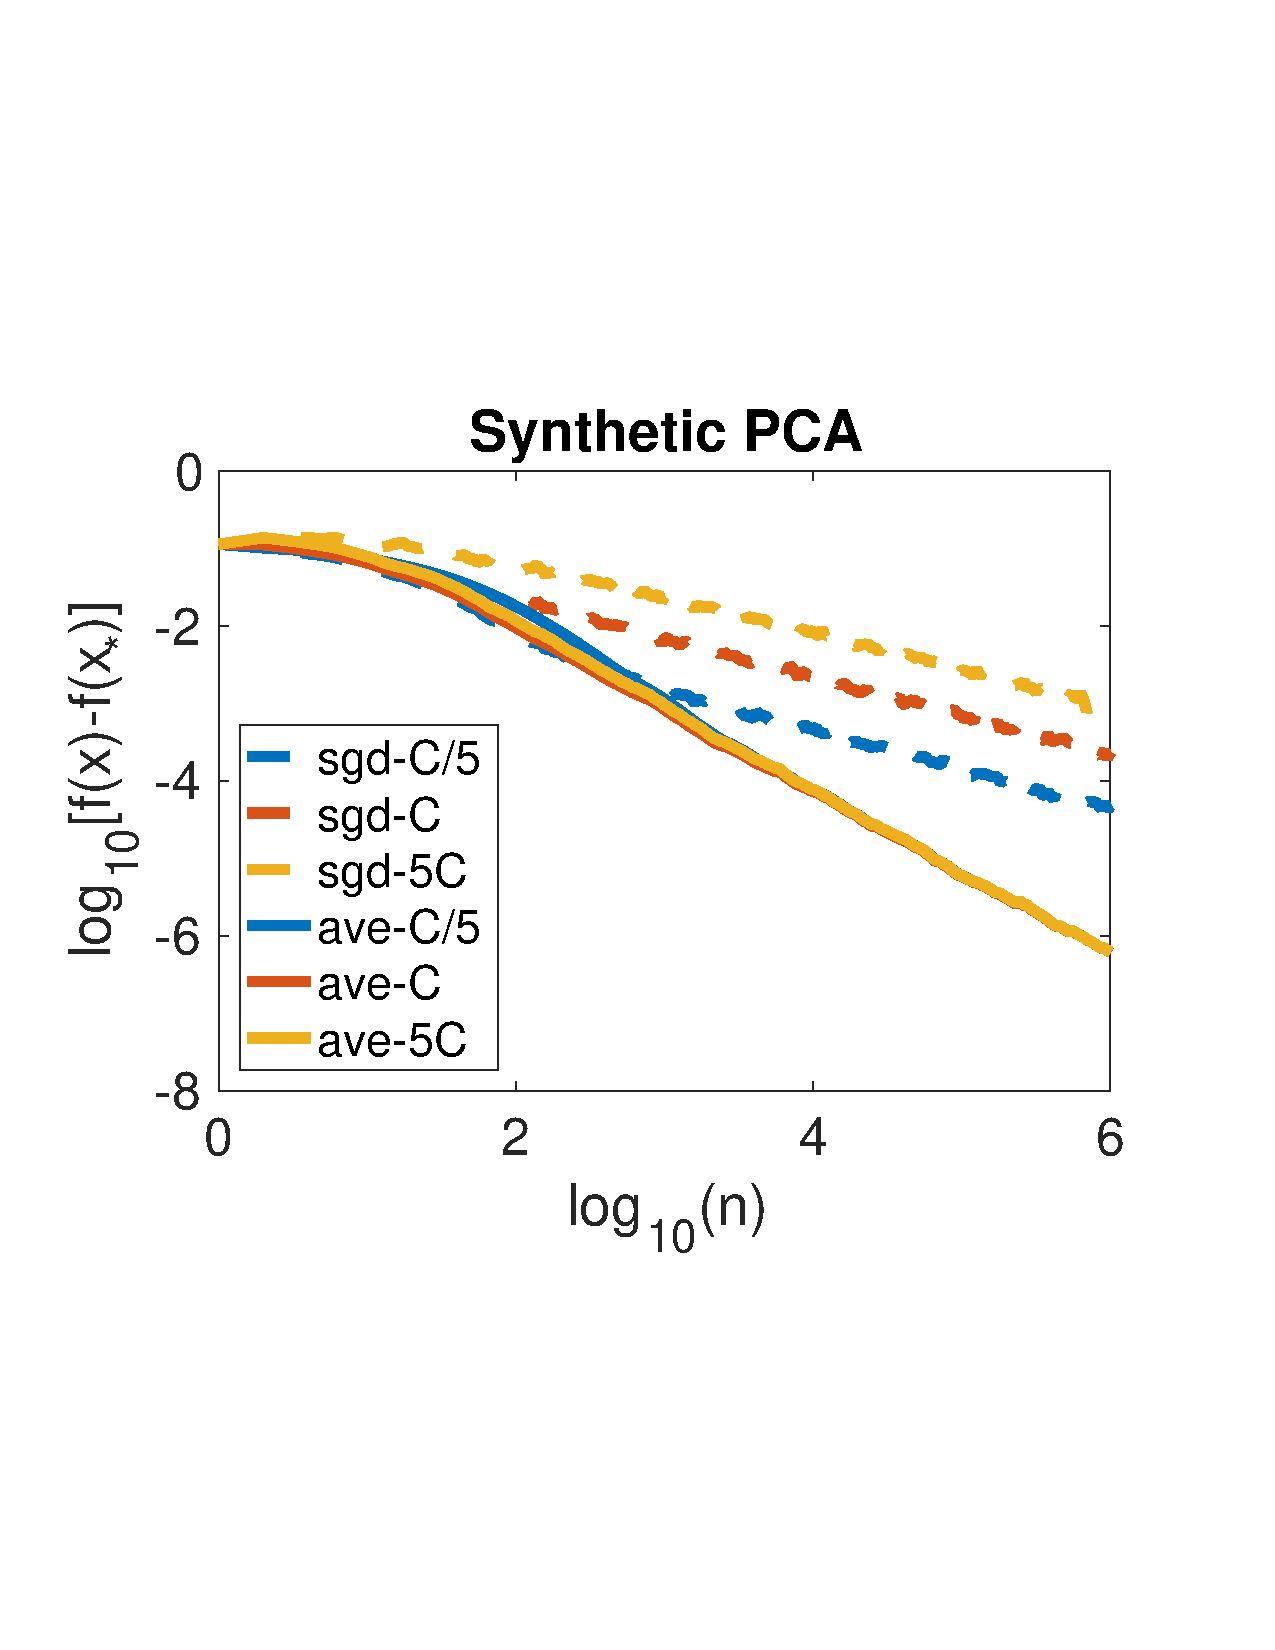
\includegraphics[width=\linewidth]{Figs/dftcc}
   \end{minipage}
   \hspace*{-10pt}
   \begin{minipage}[c]{.45\linewidth}
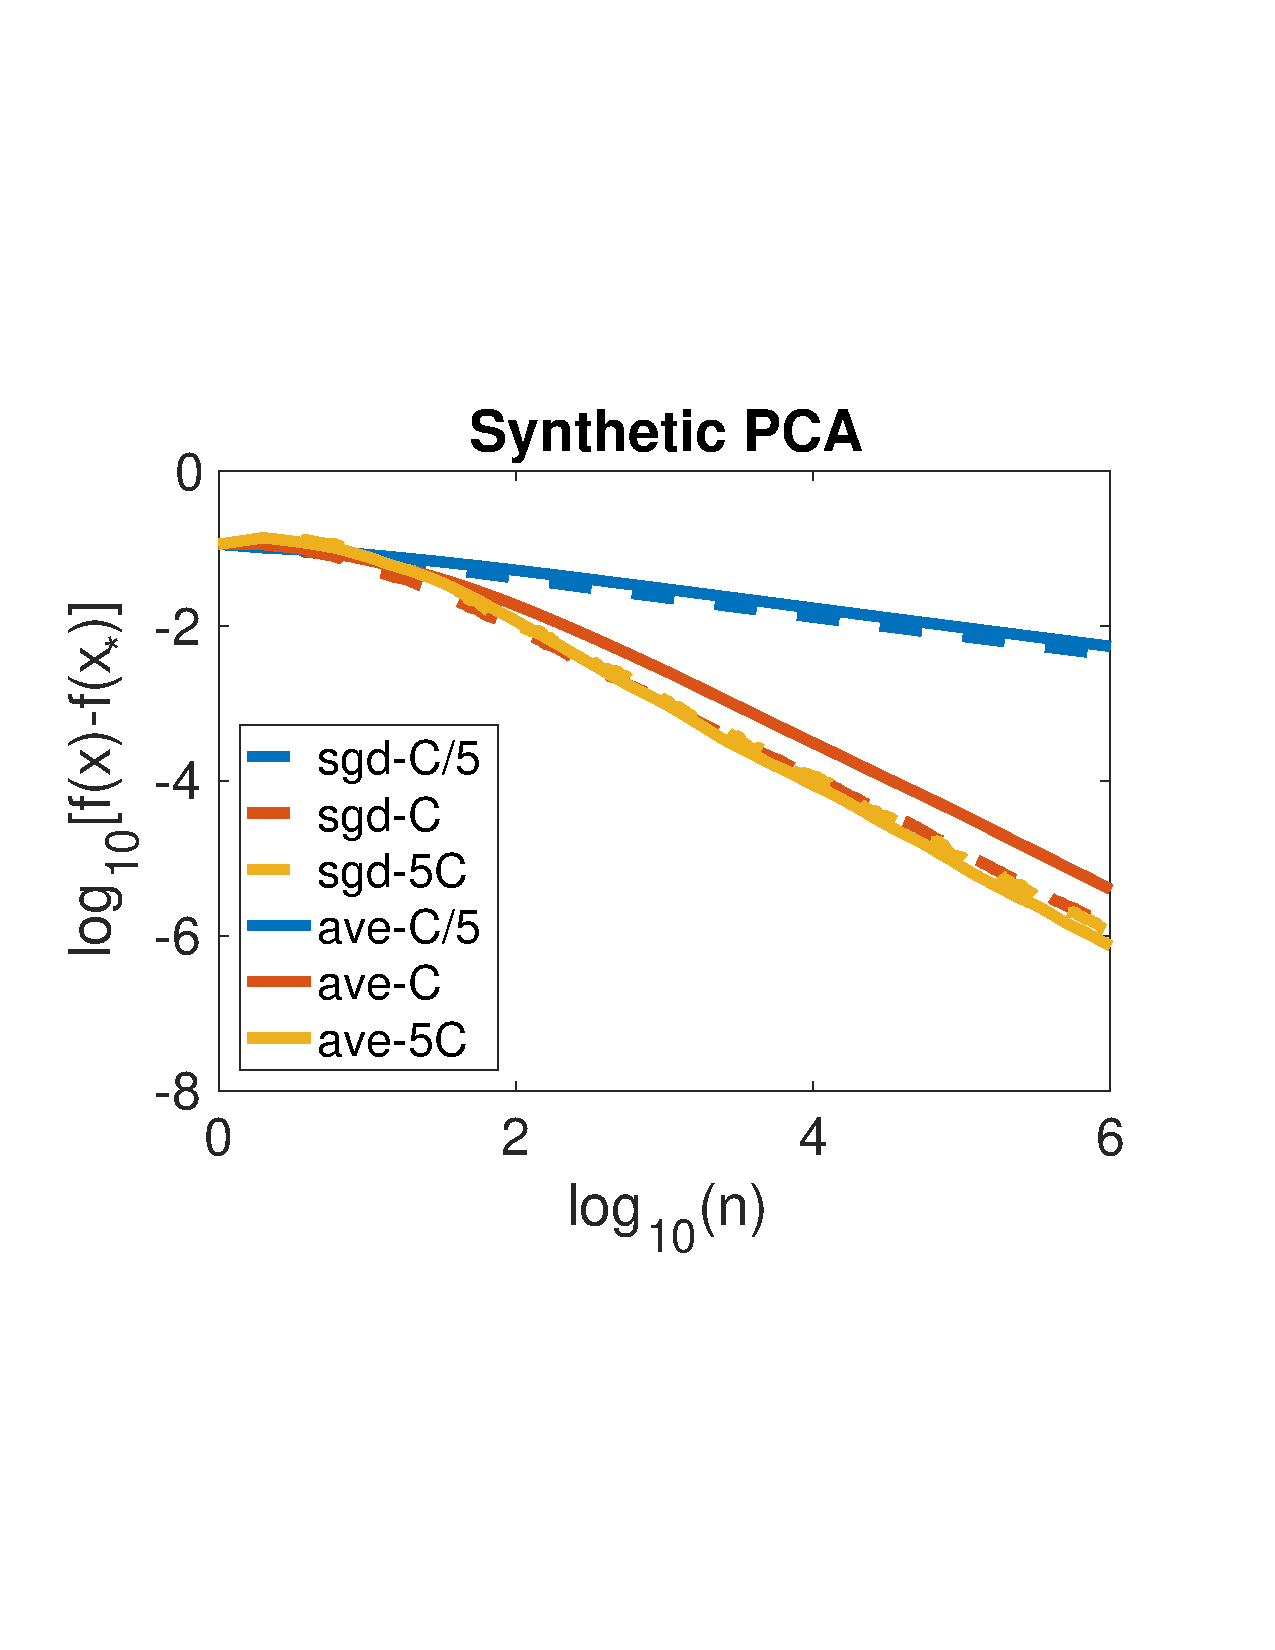
\includegraphics[width=\linewidth]{Figs/dfftc}
   \end{minipage}
   \vspace{-2.3cm}
  \caption{Robustness to constant in step size. Left:
   step size proportional to $n^{\!-\!1/2}$. Right:
   step size proportional to $n^{\!-\!1}$.}
     \label{fig:syntheticrob}
      \vspace{-0.8cm}
\end{figure}
Here, we illustrate our results on a synthetic, streaming $k$-PCA problem using the SGD algorithm defined in \eq{robust_oja}. We take $k\!\!=\!\!10$ and $d\!\!=\!\!50$. The stream $H_n\!\!\in\!\!\mathbb{R}^d$ is normally-distributed with a covariance matrix $H$ with random eigenvectors, and eigenvalues decaying as $1/i^\alpha\!+\!\beta$, for $i\leq k$, and $1/(i\!-\!1)^\alpha$, for $i>k$ and $\alpha,\beta\geq0$. All results are averaged over ten repetitions.
 \paragraph{Robustness to Conditioning.} \vspace{-6pt}
 In \myfig{synthetic} we consider two covariance matrices with different conditioning and we compare the behavior of SGD and averaged SGD for different step sizes (constant (cst), proportional to $1/\sqrt{n}$ (-1/2) and  $1/n$ (-1)). When the covariance matrix is well-conditioned, with a large eigengap (left plot), we see that SGD converges at a rate which depends on the step size whereas averaged SGD converges at a $O(1/n)$ rate independently of the step-size choice.  For poorly conditioned problems (right plot), the convergence rate deteriorates to $1/\sqrt{n}$ for non-averaged SGD with step size $1/\sqrt{n}$, and averaged SGD with both constant and $1/\sqrt{n}$ step sizes. The $1/n$ step size performs poorly with and without averaging.
 \vspace{-6pt}
\paragraph{Robustness to Incorrect Step-Size.} In \myfig{syntheticrob} we consider a well-conditioned problem and compare the behavior of SGD and averaged SGD with step size proportional to $C/\sqrt n$ and $C/n$ to investigate the robustness to the choice of the constant $C$. For both algorithms we take three different constant prefactors $C/5$, $C$ and $5C$. For the step size proportional to $C/\sqrt n$ (left plot), both SGD and averaged SGD are robust to the choice of $C$. For SGD, the iterates eventually converge at a  $1/\sqrt{n}$ rate, with a constant offset proportional to $C$. However, averaged SGD enjoys the fast rate $1/n$ for all choices of $C$. For the step size proportional to $C/n$ (right plot), if $C$ is too small, the rate of convergence is extremely slow for SGD and averaged SGD.

